\chapter{Factory Pattern }
\section{Factory Pattern – Factory method}
\subsection{Định nghĩa}

Factory Method Design Pattern hay gọi ngắn gọn là Factory Pattern là một trong những Pattern thuộc nhóm Creational Design Pattern. Factory Pattern xác định một interface để tạo một đối tượng, nhưng cho phép các lớp con quyết định lớp nào sẽ khởi tạo.  Factory Pattern giao việc khởi tạo một đối tượng cụ thể cho lớp con.

Factory Pattern đúng nghĩa là một nhà máy, và nhà máy này sẽ “sản xuất” các đối tượng theo yêu cầu của chúng ta.

\subsection{Mục đích sử dụng}
Mục đích và lợi ích:
\begin{itemize}
\item	Factory Pattern giúp giảm sự phụ thuộc giữa các module (loose coupling): cung cấp 1 hướng tiếp cận với Interface thay thì các implement. Giúp chuơng trình độc lập với những lớp cụ thể mà chúng ta cần tạo 1 đối tượng, code ở phía client không bị ảnh hưởng khi thay đổi logic ở factory hay sub class.
\item Mở rộng code dễ dàng hơn: khi cần mở rộng, chỉ việc tạo ra sub class và implement thêm vào factory method.
\item Khởi tạo các Objects mà che giấu đi xử lí logic của việc khởi tạo đấy. Người dùng không biết logic thực sực được khởi tạo bên dưới phương thức factory.
\item Dễ dạng quản lý life cycle của các Object được tạo bởi Factory Pattern.
\item Thống nhất về naming convention: giúp cho các developer có thể hiểu về cấu trúc source code.
\end{itemize}

\subsection{Mô hình câu trúc}
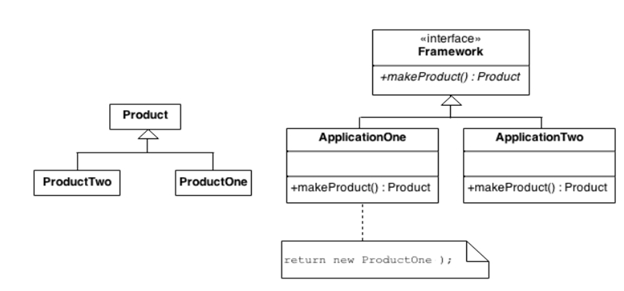
\includegraphics{GALLEYS/images/chapter5/diagram1}\\
\textbf{mô tả mô hình} : Product là obj cần phải khởi tạo, Framework là factory và Application là nơi quyết định xem đối tượng nào khởi tạo.\\
VD:\\
Giả sử trong một của hàng pizza, khách hàng muốn order 1 loại pizza, chúng có nhiểu loại, chúng ta xé quản lí những loại pizza đó một cách hợp lí. Hãy quan sát đoạn code để làm rõ vấn đề hơn, nhưng có một vấn đề là mỗi một vùng miền lại có một kiểu Pizza khác nhau,thương mại khác nhau. Cùng quan sát vấn đề:\\

Trong facory method những vấn đề liên quan đến tạo đối tượng sẽ được tạo một lớp riêng, cụ thể là một lớp trừu tượng.\\

\begin{center}
	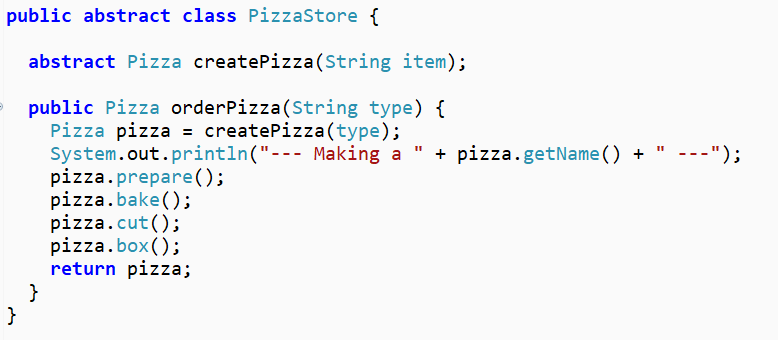
\includegraphics[width=1\columnwidth]{GALLEYS/images/chapter5/images1}
\end{center}
Đây là class PizzaStore :\\

Phương thức abstract createPizza() với phạm vi là protected dùng để xử lí việc tạo đối tượng và gói nó trong một lớp con. Điều này tách client code ra khỏi code tạo object dưới subclass.\\

Trong phương thức public orderPizza() sẽ có một biến Pizza để khởi tạo chiếc bánh mà khách hàng muốn đặt.\\

Các phương thức prepare(),bake(),cut(),box() thuộc về lớp pizza, nó là các thay đổi trên chiếc bánh.\\

Mỗi cửa hàng pizza ở mỗi vùng miền cũng khác nhau. Chúng sẽ được kế thừa từ lớp cơ sở PizzaStore.\\

\begin{center}
	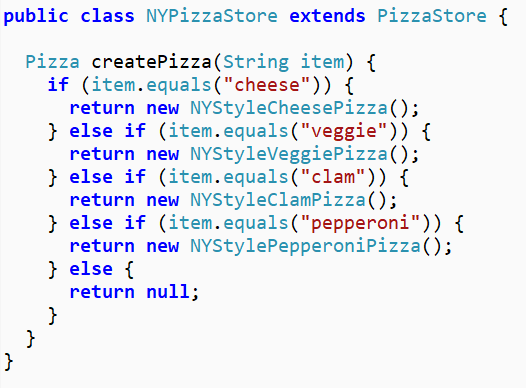
\includegraphics{GALLEYS/images/chapter5/images2}
\end{center}
Đây là một cửa hàng pizza NY\\
\begin{center}
	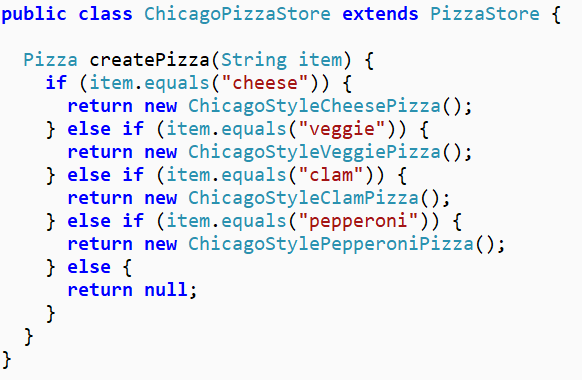
\includegraphics{GALLEYS/images/chapter5/images3}
\end{center}
\newpage
\begin{multicols}{2}
	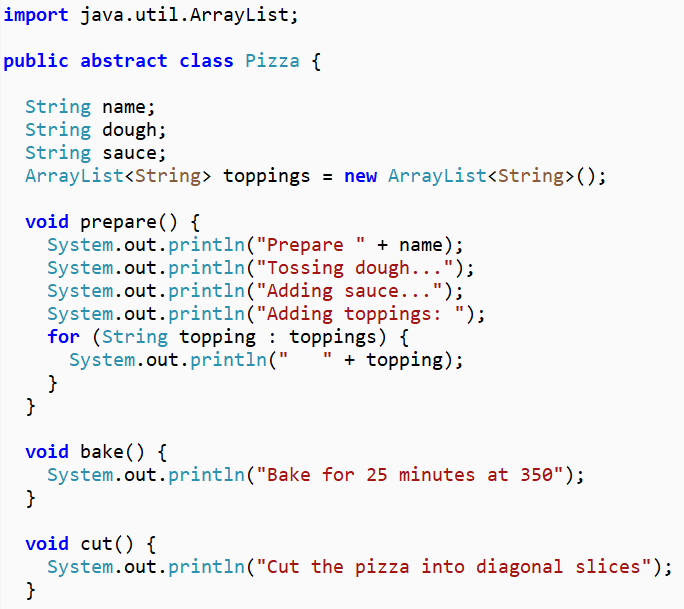
\includegraphics[width=1\columnwidth]{GALLEYS/images/chapter5/images4}
	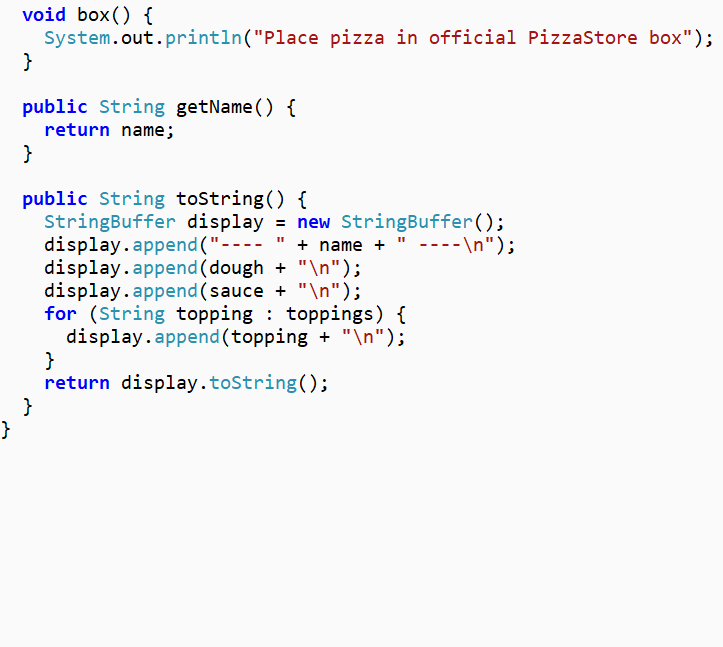
\includegraphics[width=1\columnwidth]{GALLEYS/images/chapter5/images5}
\end{multicols}

Lớp pizza này gồm các topping đi kèm của chiếc bánh.\\
Mỗi pizza có một loại tên(name), một loại bootk(dough), một loại nước sauce, và những loại topping đi kèm riêng biệt.\\

Ở đây chúng ta sử dụng StringBuffer để in ra thông tin của chiếc bánh đó.
mỗi pizza của mỗi vùng miền cụ thể có thể có cách làm khác nhau, chúng sẽ được kế thừa từ lớp Pizza.

\begin{multicols}{2}
	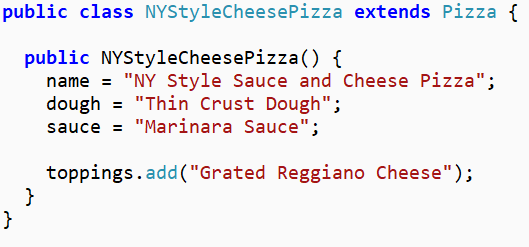
\includegraphics[width=1\columnwidth]{GALLEYS/images/chapter5/images6}
	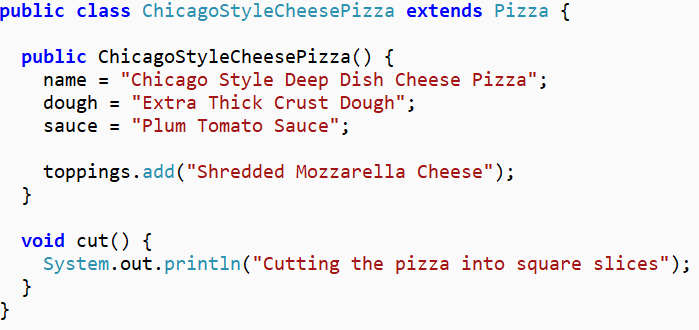
\includegraphics[width=1\columnwidth]{GALLEYS/images/chapter5/images7}
\end{multicols}
Nhận xét: ở đây chúng ta có thể thấy đoạn code này phân thành 2 class với nhiệm vụ rõ ràng, đó là Product Classes có nhiệm vụ phát triển chiếc bánh và Creator Classes với nhiệm vụ createPizza() quyết định xem chiếc bánh pizza được phát triển như thế nào .\\
Đây là kết quả:

\begin{center}
	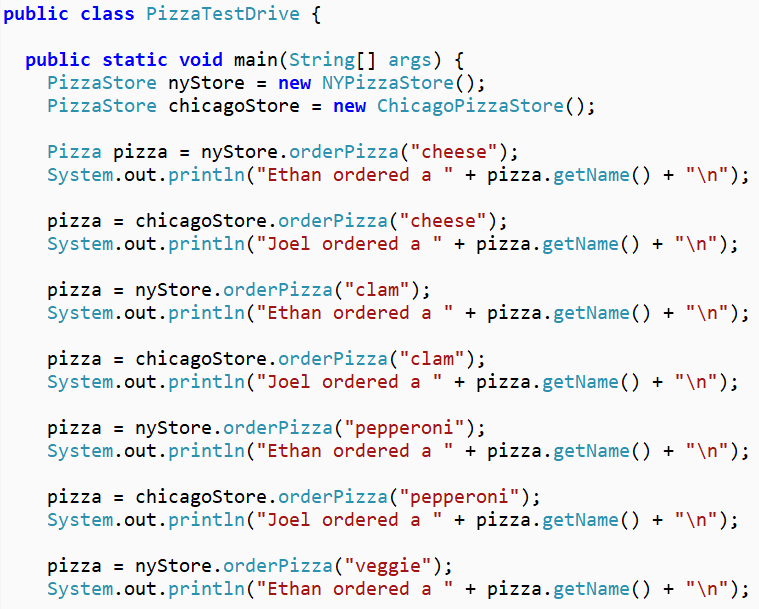
\includegraphics[height=.55\textheight]{GALLEYS/images/chapter5/images8}
	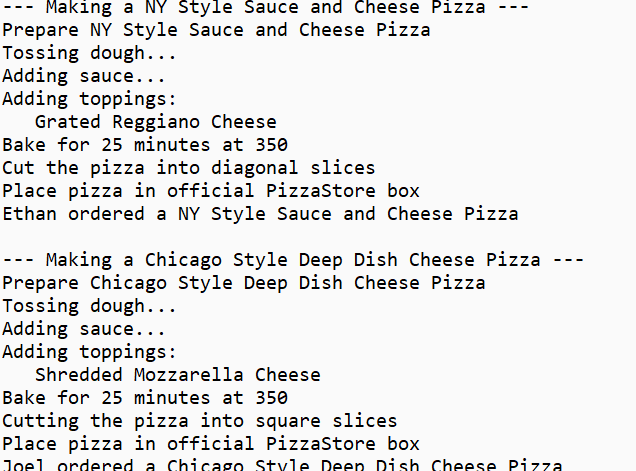
\includegraphics[height=.4\textheight]{GALLEYS/images/chapter5/images9}
\end{center}

\subsection{Factory Pattern trong thực tế}
Factory Pattern được sử dụng khi:

\begin{itemize}
	\item Chúng ta có một super class với nhiều class con và dựa trên đầu vào, chúng ta cần trả về một class con. Mô hình này giúp chúng ta đưa trách nhiệm của việc khởi tạo một lớp từ phía người dùng (client) sang lớp Factory.
	\item Chúng ta không biết sau này sẽ cần đến những lớp con nào nữa. Khi cần mở rộng, hãy tạo ra sub class và implement thêm vào factory method cho việc khởi tạo sub class này.\\
	Bạn có thể thấy Factory Pattern được áp dụng trong:
	\item JDK: java.util.Calendar, ResourceBundle, NumberFormat, …
	\item BeanFactory trong Spring Framework.
	\item SessionFactory trong Hibernate Framework.
\end{itemize}
Bạn có thể thấy Factory Pattern được áp dụng trong:
\begin{itemize}
	\item JDK: java.util.Calendar, ResourceBundle, NumberFormat, …
	\item BeanFactory trong Spring Framework.
	\item SessionFactory trong Hibernate Framework.
\end{itemize}

\section{Factory Pattern – Abstract Factory method}
\subsection{Định nghĩa}

Abstract Factory pattern là một trong những Creational pattern. Nó là phương pháp tạo ra một Super-factory dùng để tạo ra các Factory khác. Hay còn được gọi là Factory của các Factory. Abstract Factory Pattern là một Pattern cấp cao hơn so với Factory Method Pattern.

\subsection{Mục đích sử dụng}
Mục đích và lợi ích:
\begin{itemize}
	\item	Các lợi ích của Factory Pattern cũng tương tự như Factory Method Pattern như: cung cấp hướng tiếp cận với Interface thay thì các implement, che giấu sự phức tạp của việc khởi tạo các đối tượng với người dùng (client), độc lập giữa việc khởi tạo đối tượng và hệ thống sử dụng, …
	\item   Giúp tránh được việc sử dụng điều kiện logic bên trong Factory Pattern. Khi một Factory Method lớn (có quá nhiều sử lý if-else hay switch-case), chúng ta nên sử dụng theo mô hình Abstract Factory để dễ quản lý hơn (cách phân chia có thể là gom nhóm các sub-class cùng loại vào một Factory).
	\item   Abstract Factory Pattern là factory của các factory, có thể dễ dạng mở rộng để chứa thêm các factory và các sub-class khác.
	\item 	Dễ dàng xây dựng một hệ thống đóng gói (encapsulate): sử dụng được với nhiều nhóm đối tượng (factory) và tạo nhiều product khác nhau.
\end{itemize}

\subsection{Mô hình câu trúc}
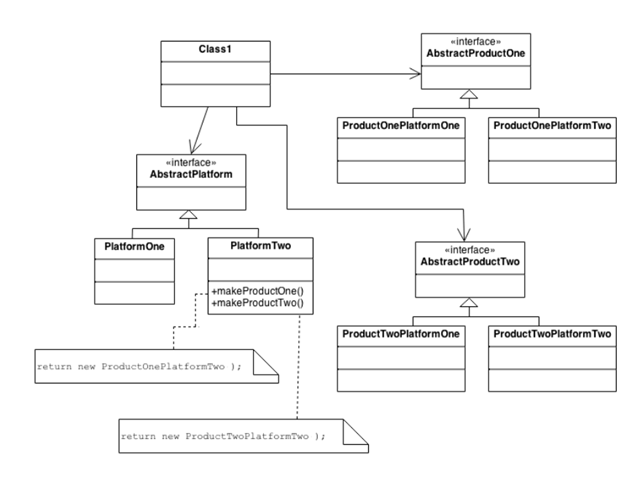
\includegraphics{GALLEYS/images/chapter5/diagram2}\\
\textbf{AbstractFactory}: Khai báo dạng interface hoặc abstract class chứa các phương thức để tạo ra các đối tượng abstract.\\
\textbf{ConcreteFactory}: Xây dựng, cài đặt các phương thức tạo các đối tượng cụ thể.\\
\textbf{AbstractProduct}: Khai báo dạng interface hoặc abstract class để định nghĩa đối tượng abstract.\\
\textbf{Product}: Cài đặt của các đối tượng cụ thể, cài đặt các phương thức được quy định tại AbstractProduct.\\
\textbf{Client}: là đối tượng sử dụng AbstractFactory và các AbstractProduct.\\
VD:\\

Như ở phần Factory method đã có ví dụ về chuỗi cửa hàng pizza, giờ đây chúng ta sẽ phát triển chúng:\\

Do mỗi loại bánh sẽ có nguyên liệu khác nhau vd: Chicago sẽ là một loại nguyên liệu khác so với New York.\\

Do đó chúng ta sẽ cần tạo ra một bộ nguyên liệu :\\


\begin{center}
	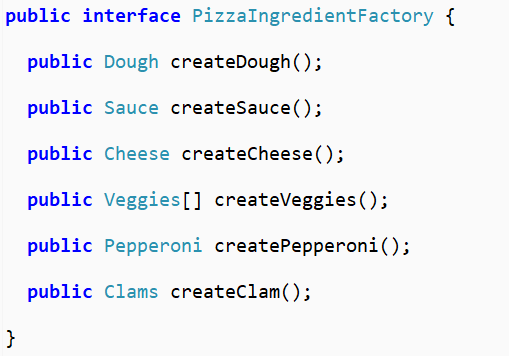
\includegraphics{GALLEYS/images/chapter5/images10}
\end{center}
Do tính vùng miền, lớp con sẽ được implement từ PizzaIngredientFactory.\\
Implement một tập hợp các lớp nguyên liệu sẽ được sử dụng như ReggianoCheese, RedPeppers và ThickCrustDough. Các lớp này có thể được chia sẻ giữa các khu vực khi thích hợp. \\
Sau đó, chúng ta cần kết nối tất cả những điều này bằng cách đưa các nhà máy sản xuất nguyên liệu mới vào PizzaStore.\\


\begin{center}
	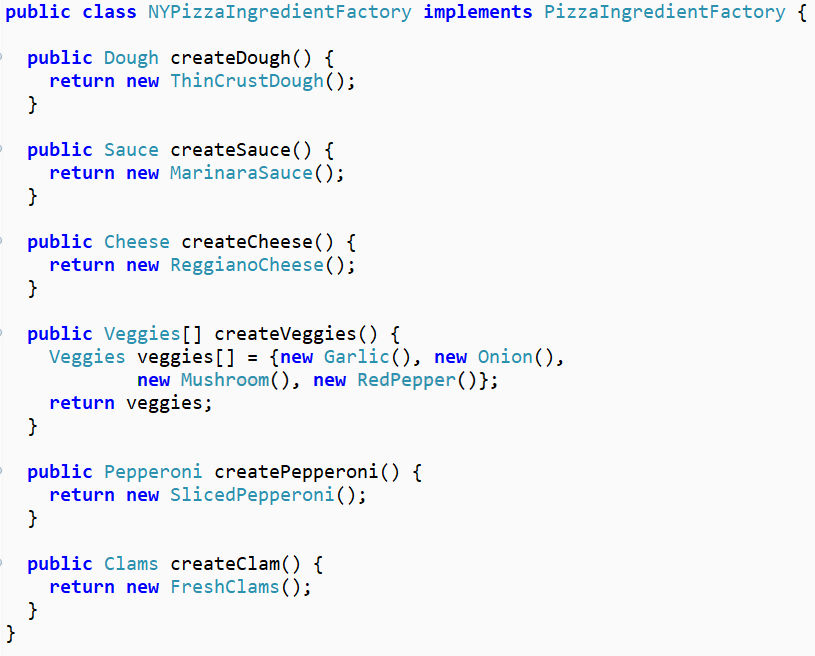
\includegraphics{GALLEYS/images/chapter5/images11}
\end{center}
Phương thức createDough() trả về kiểu bột để làm bánh.\\
Tuong tự chúng ta có createSauce(), createCheese(), createVeggies() , createPepperoni() ..v..v..\\
Phương thức createVeggies() trả về một mảng các loại rau củ.\\
Khi đó sẽ có thay đổi trên lớp Pizza:\\

\begin{center}
	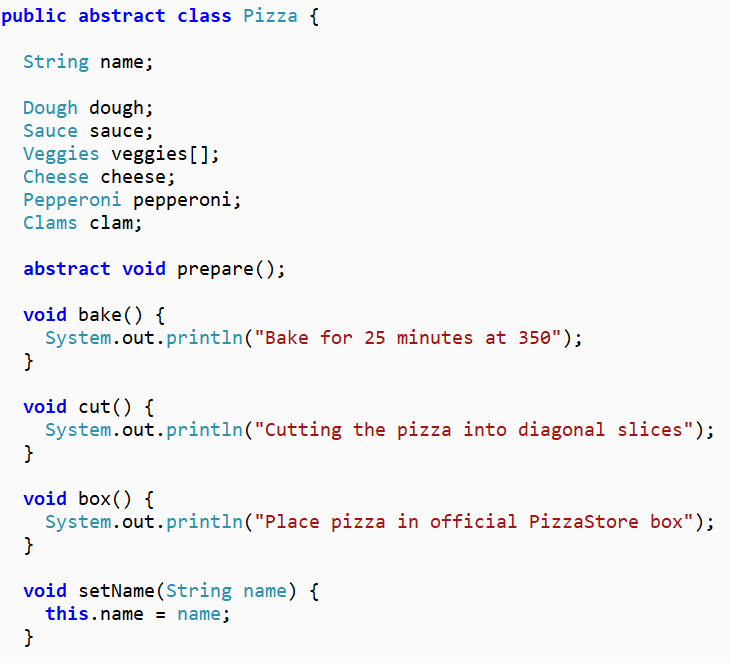
\includegraphics{GALLEYS/images/chapter5/images12}
\end{center}
Bây giờ chiếc bánh đã linh động hơn về việc chuẩn bị gia vị.
\begin{center}
	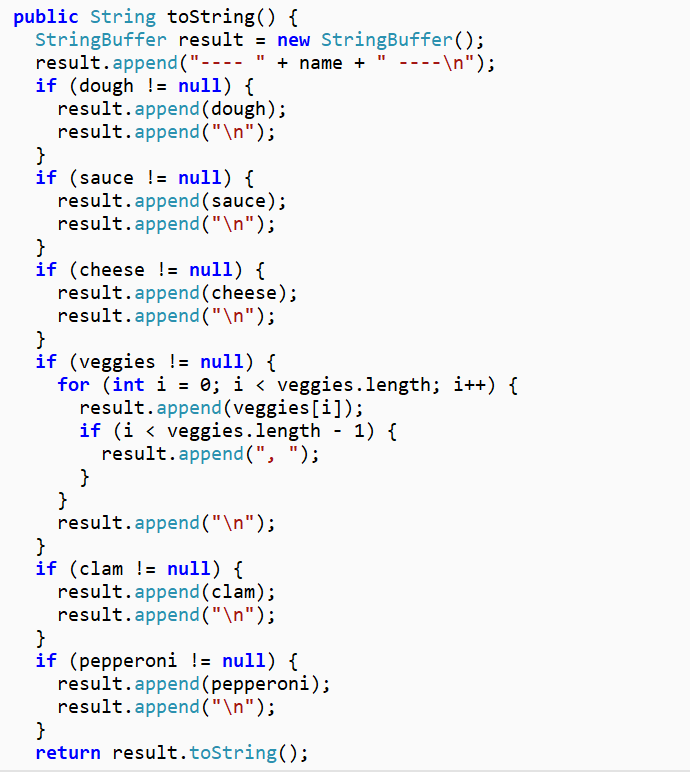
\includegraphics{GALLEYS/images/chapter5/images13}
\end{center}

Lớp con của Pizza lúc này cũng đã có sự thay đổi:

\begin{center}
	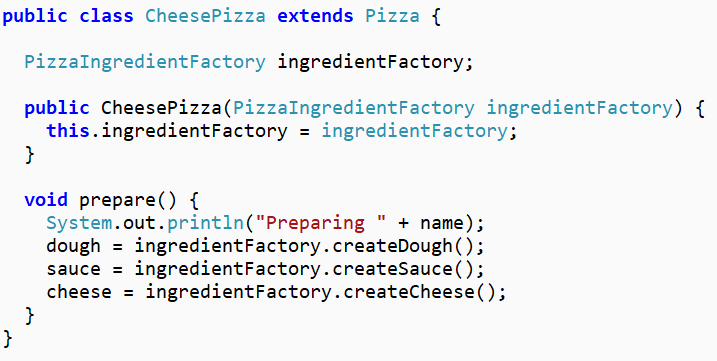
\includegraphics{GALLEYS/images/chapter5/images14}
\end{center}

Từ những thay đổi trên chúng ta cùng khám phá cửa hàng pizza mới sau khi sửa đổi:\\
\begin{center}
	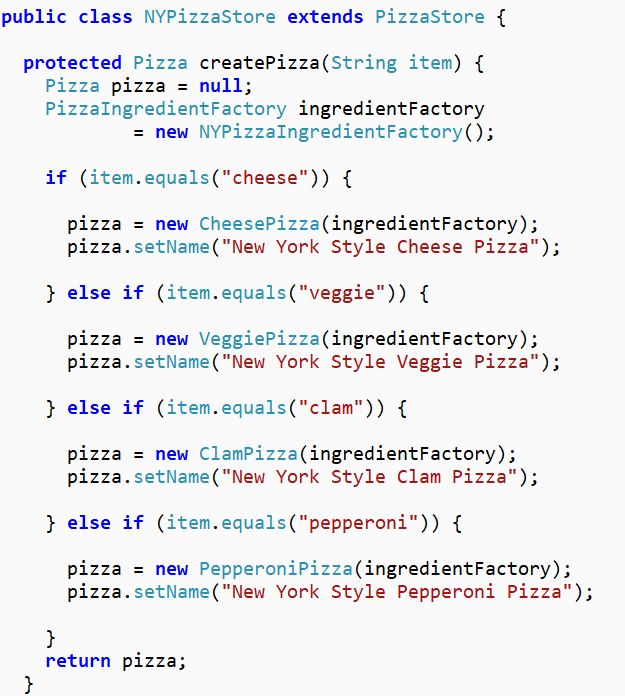
\includegraphics[height=.55\textheight]{GALLEYS/images/chapter5/images15}
\end{center}
Và đây là kết quả :\\
\begin{center}
	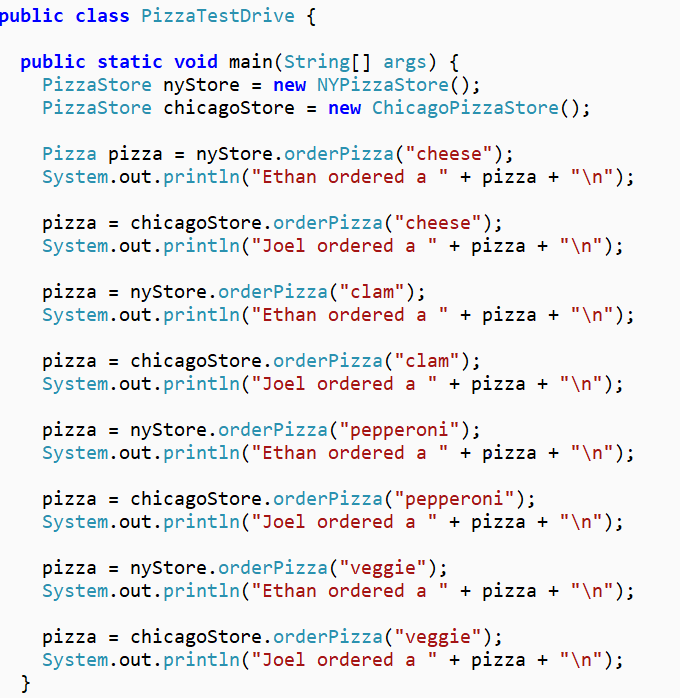
\includegraphics{GALLEYS/images/chapter5/images16}
\end{center}
\begin{center}
	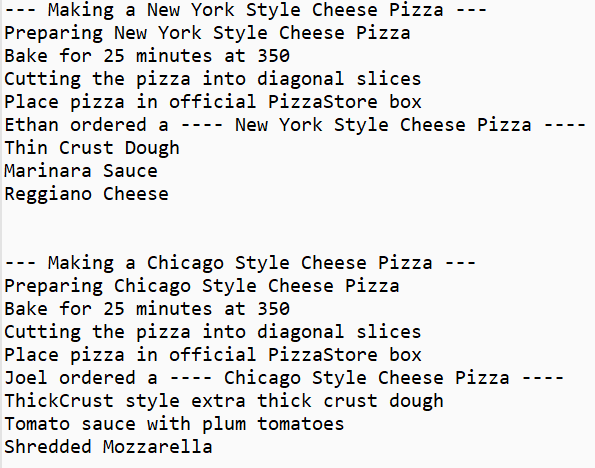
\includegraphics{GALLEYS/images/chapter5/images17}
\end{center}
Chúng ta cũng cần cung cấp cho cửa hàng một tham chiếu (reference) đến các nhà máy sản xuất nguyên liệu của địa phương của họ (Chicago sẽ có ChicagoPizzaIngredientFactory, NY sẽ có NYPizzaIngredientFactory…)\\
Abstract Factory Pattern cho phép client sử dụng giao diện trừu tượng để tạo ra một bộ sản phẩm liên quan mà không cần biết (hoặc quan tâm) về các sản phẩm cụ thể được tạo ra thực sự\\
